\hypertarget{(chap:capitolo6)}{}
\chapter{Risultati sperimentali}
In questo capitolo vedremo i risultati sperimentali per ogni metodo, vedremo prima quelli applicati alle matrici grezze, poi quelli basati sulla combinazione delle stesse, i risultati dell'approccio next-based per concludere infine con un confronto critico dei risultati.
\section{Risultati preprocessing matrici grezze}
Nelle sezioni successive saranno riportati i risultati delle valutazioni di ciascun modello rispetto la metrica $AUC$ e la $NDCG$ con $k\in \{5, 10, 25, 100\}$.
La metrica che riteniamo sia più significativa è la $NDCG$ in quanto si basa sul ranking degli item nella lista $TopN$, per i confronti abbiamo scelto di usare $k=25$.\\
Come riportato nel capitolo precedente la valutazione sarà condotta in due fasi: 
\begin{enumerate}
    \item preliminare: confrontiamo i risultati dei modelli (MF, UserKnn) con parametri di default applicati alle matrici dei rating con il valore soglia dato dal modello MostPop, il tutto usando il validation set;
    \item avanzata: dopo aver effettuato il tuning dei modelli con le matrici rimanenti, si confrontano i risultati con il bound dato dal VAECF usando il test set.
\end{enumerate} 

\subsection{Risultati soglia}
In questa sezione vedremo i risultati del modello MostPop e del VAECF, che verranno utilizzati come bound per valutare quelli succcessivi. 

\subsubsection{MostPop}
Come detto il modello MostPop restituisce per ogni user la stessa lista di item più popolari e nella tabella \ref{tab:mostpop_val} ne riportiamo i risultati sul validation set.
\begin{center}
\begin{tabular}{|l|c|cccc|}
    \toprule
    $dataset$ &    $AUC$ &  $NDCG@5$ & $NDCG@10$  & $NDCG@25$ & $NDCG@100$  \\
    \midrule
    macchine & 0.7644 & 0.0920 & 0.1263 & 0.1647 &  0.2414 \\
    ricambi  & 0.3427 & 0.0000 & 0.0299 & 0.0358 &  0.0732 \\
    totale   & 0.2810 & 0.0360 & 0.0733 & 0.0627 &  0.0811 \\
\bottomrule
\end{tabular}
\captionof{table}{Risultati modello MostPop per tipo dataset sul validation set}
\label{tab:mostpop_val}
\end{center} 

Useremo questi risultati come soglia per la fase preliminare, testando i risultati delle matrici applicate ai modelli MF e UserKnn. Nel caso in cui questi siano migliori, si procederà al tuning dei parametri del modello stesso e al calcolo finale dei risultati sul test set.\\
Quelli riportati nella tabella \ref{tab:mostpop_test} sono i risultati del MostPop sul test set.\\
\begin{center}
\begin{tabular}{|l|c|cccc|}
    \toprule
    $dataset$ &    $AUC$ &  $NDCG@5$ & $NDCG@10$  & $NDCG@25$ & $NDCG@100$  \\
    \midrule
    macchine & 0.7897 & 0.1001 &  0.1364 &  0.1875 & 0.2610 \\
    ricambi  & 0.3924 & 0.0619 &  0.0753 &  0.0793 & 0.1365 \\
    totale   & 0.3101 & 0.0944 &  0.0807 &  0.0866 & 0.1281 \\
\bottomrule
\end{tabular}
\captionof{table}{Risultati modello MostPop per tipo dataset sul test set}
\label{tab:mostpop_test}
\end{center}

\subsubsection{VAECF}
Il modello VAECF è un modello che funziona su rating impliciti, la fase preliminare ha richiesto il tuning dei parametri riportati di seguito:
\begin{itemize}
    \item $n_{int}$ è la dimensione della rappresentazione latente interna, i possibili valori sono $\{5,10,15,20,50\}$;
    \item $n_{hid}$ è il numero di neuroni del layer dell'encoder e del decoder, i valori possibili sono $\{10,20,30,50,100,200\}$;
    \item $f_{act}$ è la funzione di attivazione applicata nei layer nascosti, che può essere una delle seguenti $\{sigmoid, tanh, elu, relu, relu6\}$.
\end{itemize}
\begin{minipage}[H]{0.45\textwidth}
    \begin{center}
        \begin{tabular}{|l|ccc|}
            \toprule
            $dataset$ &    $n_{int}$ &  $n_{hid}$ & $f_{act}$ \\
            \midrule
            macchine & 5 & 30 & relu \\
            ricambi  &	5 & 30 & sigmoid\\
            totale  & 5 & 30 & sigmoid\\
        \bottomrule
        \end{tabular}
        \captionof{table}{Parametri selezionati.}
        \label{tab:tuning_vaecf}
\end{center}
\end{minipage}
\begin{minipage}[H]{0.55\textwidth}
    Il tuning dei parametri ha portato a considerare tutte le possibili combinazioni degli stessi, vediamo per ogni dataset quali valori hanno restituito i risultati migliori sul validation set.
\end{minipage}\\

Vediamo ora i risultati suddivisi per dataset sul validation set con il modello ottimizzato nella Figura \ref{tab:vaecf_val}.
\begin{center}
\begin{tabular}{|l|c|cccc|}
    \toprule
    $dataset$ &    $AUC$ &  $NDCG@5$ & $NDCG@10$  & $NDCG@25$ & $NDCG@100$  \\
    \midrule
    macchine & 0.8201 & 0.1325 & 0.1768 & 0.2282 & 0.3032 \\
    ricambi  & 0.4773 & 0.0506 & 0.0452 & 0.0643 & 0.1052 \\
    totale   & 0.4190 & 0.1208 & 0.0980 & 0.0741 & 0.0941 \\
\bottomrule
\end{tabular}\\
\captionof{table}{Risultati VAECF ottimizzato per tipo dataset sul validation set.}
\label{tab:vaecf_val}
\end{center}
Dato che si utilizzeranno i risultati del VAECF ottimizzato sul test set come soglia nella fase avanzata, questi sono presenti in Figura \ref{tab:vaecf_test}.
\begin{center}
\begin{tabular}{|l|c|cccc|}
    \toprule
    $dataset$ &    $AUC$ &  $NDCG@5$ & $NDCG@10$  & $NDCG@25$ & $NDCG@100$  \\
    \midrule
    macchine & 0.8269 & 0.1473 &  0.1948 & 0.2487 & 0.3301 \\
    ricambi  & 0.4930 & 0.0801 &  0.0919 & 0.1075 & 0.1401 \\
    totale   & 0.4343 & 0.0988 &  0.0874 & 0.0964 & 0.1398 \\
\bottomrule
\end{tabular}
\captionof{table}{Risultati VAECF ottimizzato per tipo dataset sul test set.}
\label{tab:vaecf_test}
\end{center}

\subsection{Fase test preliminare}
In questa sezione vedremo per ogni tecnica di preprocessing applicata sulle matrici grezze i risultati ottenuti.
Cominceremo prima con la tecnica basata su min-max, poi con quella ordered-based per concludere con quella product-based. 
Spesso si farà riferimenti ai risultati dei modelli, intendendo il risultato della metrica dato dall'applicazione del modello alla matrice dei rating.
Come spiegato nei capitoli precedenti i metodi min-max e ordered-based sono applicabili a diversi gruppi di triplette, vedremo i risultati per ciascuno di essi.\\

%------------------------------------------------------------------------------------------------------------------------------------------------------


\subsubsection{Normalizzazione min-max gruppo globale}
In questa sezione vedremo la normalizzazione min-max applicata al gruppo globale, ossia quello contenente tutte le triplette.
Nel grafico composto \ref{tab:minmax_globale} possiamo vedere sulle righe i tipi di dataset (macchine, ricambi, totale), mentre sulle colonne le \textit{espressioni d'interesse}. Ciascun grafico poi mostra sulle ascisse la $scale$ della matrice dei rating e sulle ordinate il risultato ottenuto da tale matrice rispetto la metrica $NDCG@25$.
\begin{center}
    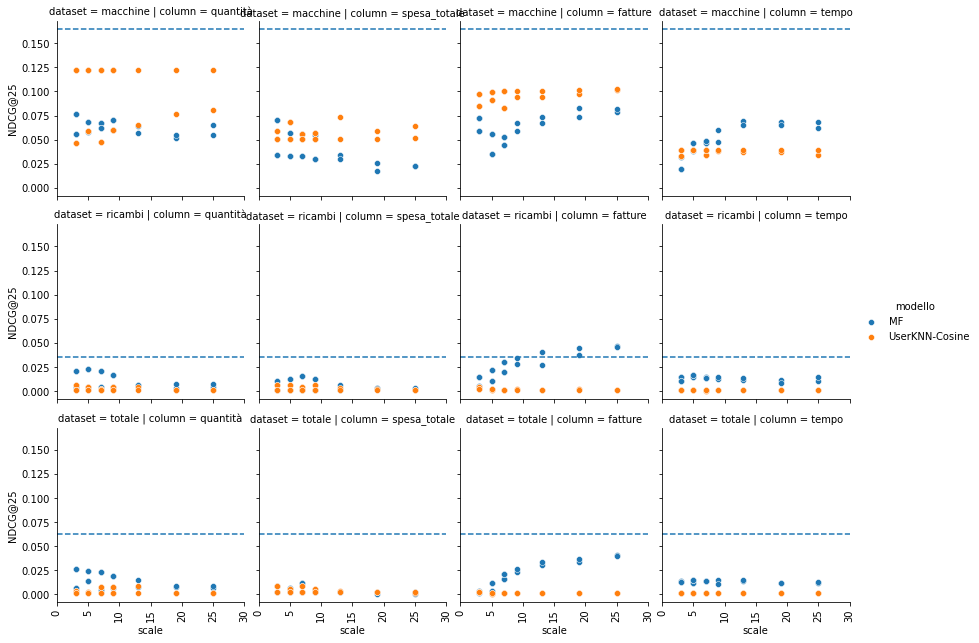
\includegraphics[width=16cm]{figures/risultati_minmax_globale.png}
    \captionof{figure}{Risultati normalizzazione min-max gruppo globale.}
    \label{tab:minmax_globale}
\end{center}
La linea tratteggiata blu rappresenta il risultato del modello MostPop che viene usato come bound.
In questo grafico composto per ogni valore della scala vengono riportati quattro puntini, per questa tecnica ogni matrice dei rating è stata tenuta sia in versione continua che in versione intera. A queste due matrici vengono applicati i modelli MF e UserKnn, da cui otteniamo quattro risultati, quelli di colore blu sono i risultati forniti dal modello MF, mentre quelli arancioni quelli del modello UserKnn.

\subsubsection{Normalizzazione min-max gruppo user-based}
In questa sezione vedremo la normalizzazione min-max applicata al gruppo user-based, ossia quello dove ciascuno di essi contiene solo le triplette di un singolo user. Il grafico composto \ref{tab:minmax_user_based} di seguito possiede la stessa struttura di quello (\ref{tab:minmax_globale}) del paragrafo precedente. Sono presenti risultati positivi nell'incrocio tipo dataset ricambi - espressione d'interesse (numero fatture).
\begin{center}
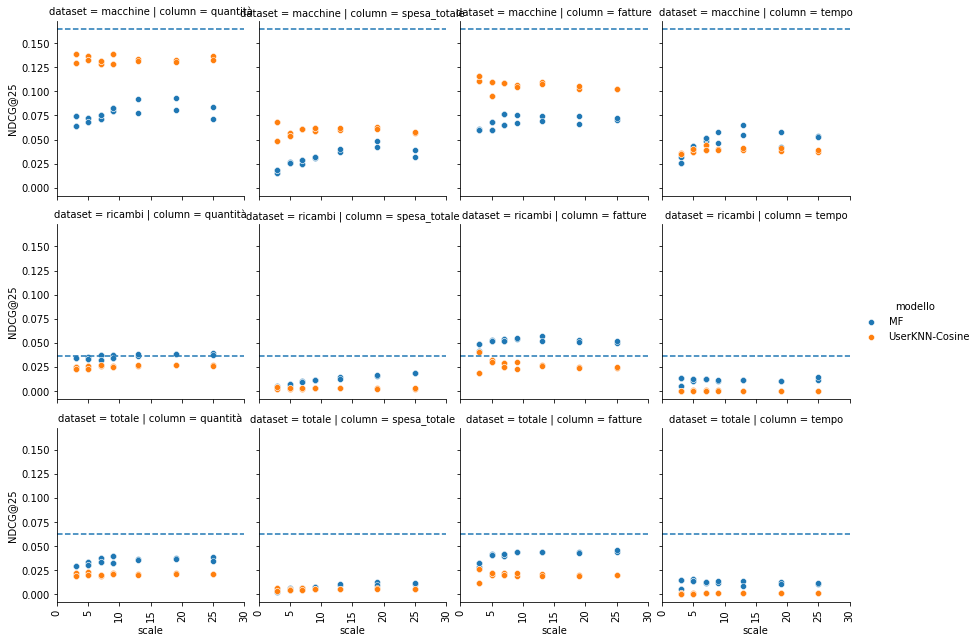
\includegraphics[width=16cm]{figures/risultati_minmax_singolo.png}
\captionof{figure}{Risultati normalizzazione min-max gruppo user-based.}
\label{tab:minmax_user_based}
\end{center}

\subsubsection{Normalizzazione min-max gruppo user-category-based}
Vediamo la normalizzazione min-max applicata al gruppo user-category-based, dove le triplette vengono divise per user e per categoria.
Le macchine hanno a disposizione solo la divisione in categorie secondo la gerarchia prodotto, mentre i ricambi possono essere divisi secondo le categorie di 2° e 3° livello della gerarchia prodotto e dal gruppo merceologico. Per il tipo dataset totale si proverà ad usare prima solo le categorie della gerarchia prodotto, poi le categorie della gerarchia prodotto solo per le macchine mentre per i ricambi le categorie del gruppo merceologico.
\paragraph{Macchine}\mbox{} \\
Come possiamo vedere dal grafico composto \ref{tab:minmax_macchine}, sulle righe abbiamo i livelli della gerarchia prodotto (1°, 2°, 3° livello), mentre sulle colonne abbiamo le espressioni d'interesse. 
Non sono presenti risultati che superino la soglia critica.
\begin{center}
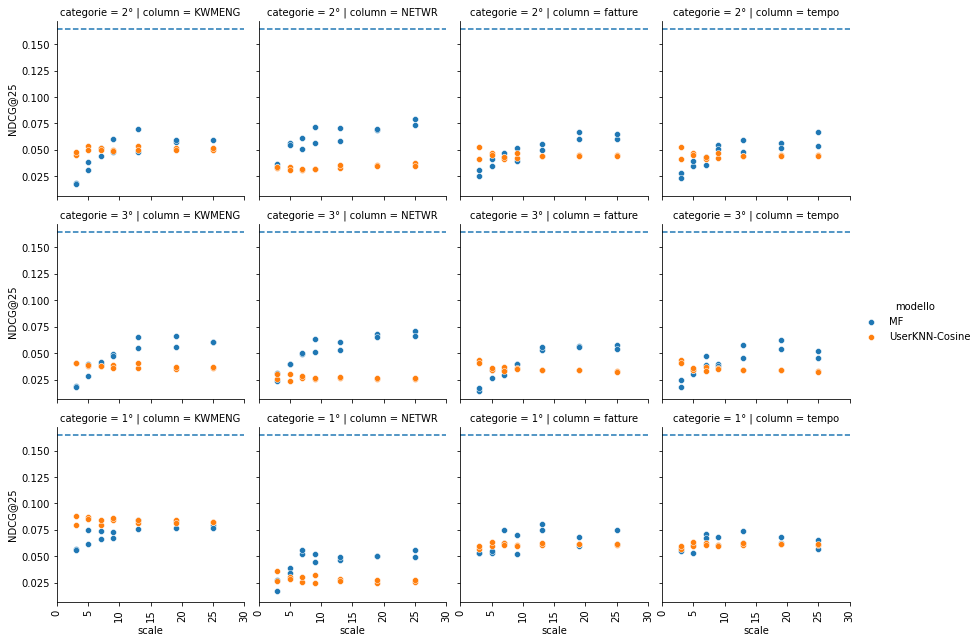
\includegraphics[width=15cm]{figures/risultati_minmax_categoria_macchine.png}
\captionof{figure}{Risultati normalizzazione min-max gruppo user-category based dataset macchine.}
\label{tab:minmax_macchine}
\end{center}
\newpage

\paragraph{Ricambi}\mbox{} \\
Come possiamo vedere dal grafico composto \ref{tab:minmax_ricambi}, sulle righe abbiamo il 1° e 2° livello della gerarchia prodotto e la divisione del gruppo merceologico (\textit{MATKL}), mentre sulle colonne abbiamo le espressioni d'interesse. Abbiamo risultati che superano la soglia critica dividendo le triplette secondo le categorie di 2° livello della gerarchia prodotto con le espressioni numero di fatture e recentezza.
\begin{center}
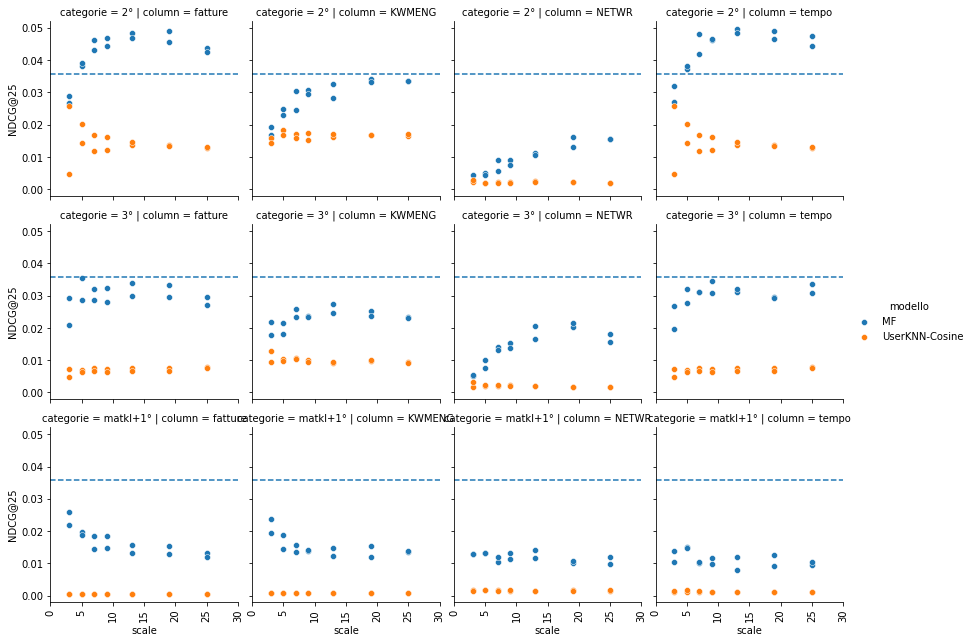
\includegraphics[width=16cm]{figures/risultati_minmax_categoria_ricambi.png}
\captionof{figure}{Risultati normalizzazione min-max gruppo user-category based dataset ricambi.}
\label{tab:minmax_ricambi}
\end{center}

\paragraph{Totale}\mbox{} \\
Come possiamo vedere dal grafico composto \ref{tab:minmax_totale} sulle righe abbiamo il 1°, 2° e 3° livello della gerarchia prodotto e successivamente le precedenti categorie applicate solo alle macchine, mentre i ricambi si sono divisi secondo il gruppo merceologico. Sulle colonne abbiamo le espressioni d'interesse. Non abbiamo alcun risultato sopra la soglia.
\begin{center}
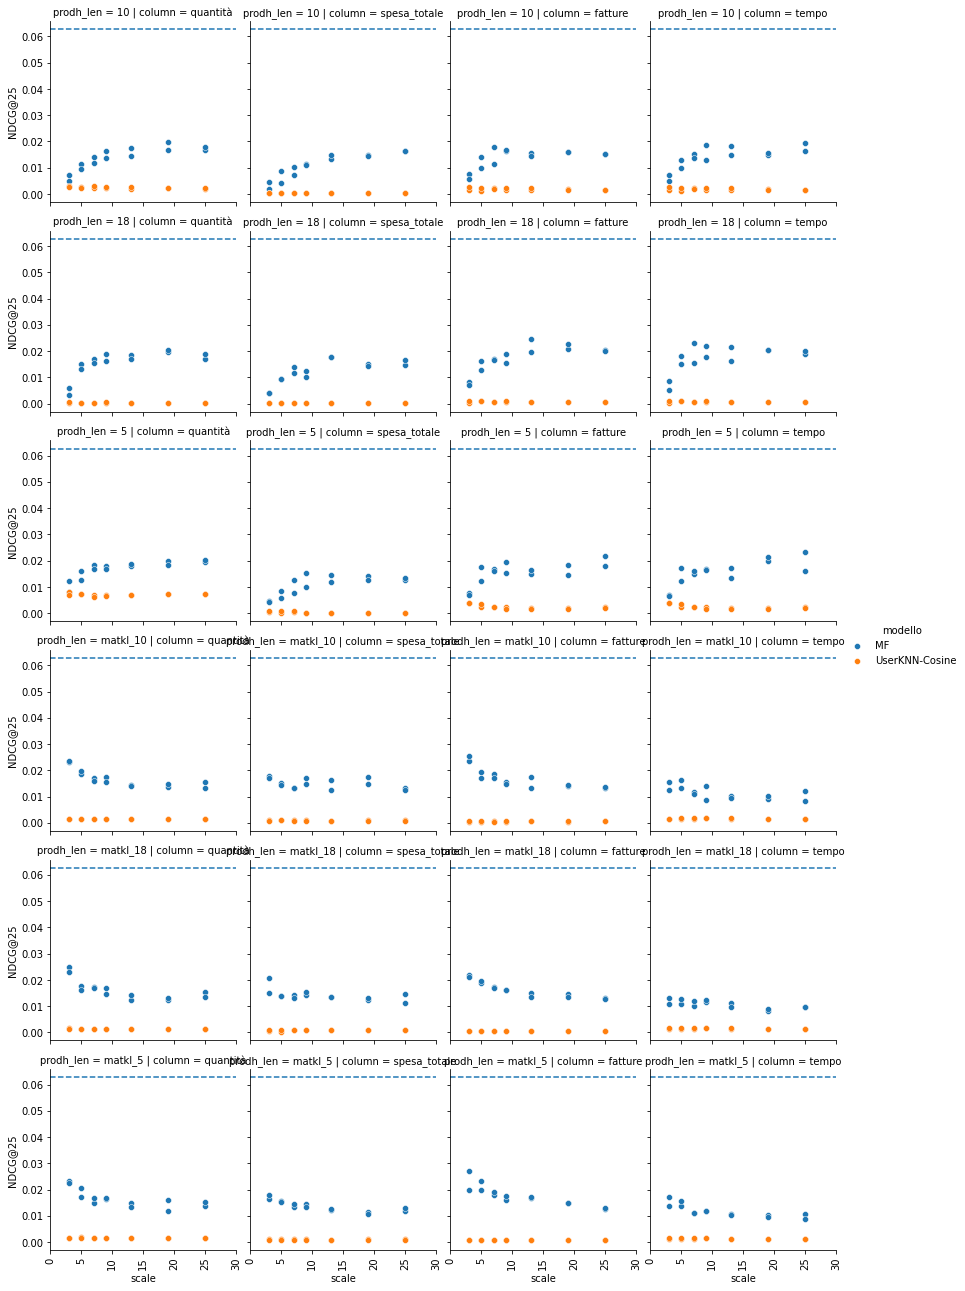
\includegraphics[width=14.5cm]{figures/risultati_minmax_categoria_totale.png}
\captionof{figure}{Risultati normalizzazione min-max gruppo user-category based dataset totale.}
\label{tab:minmax_totale}
\end{center}
%------------------------------------------------------------------------------------------------------------------------------------------------------

\subsubsection{Tecnica ordered-based gruppo globale}
In questa sezione vedremo la tecnica di preprocessing ordered-based applicata al gruppo globale, ossia quello contenente tutte le triplette.
Nel grafico composto \ref{tab:ordered_globale} sottostante possiamo vedere sulle righe i tipi di dataset (macchine, ricambi, totale), mentre sulle colonne le \textit{espressioni d'interesse}. Ciascun grafico poi mostra sulle ascisse la $scale$ della matrice dei rating e sulle ordinate il risultato ottenuto da tale matrice rispetto la metrica $NDCG@25$. \\
La linea tratteggiata blu rappresenta il risultato del modello MostPop che viene usato come bound.
In questo grafico composto per ogni valore della scala vengono riportati quattro puntini, per questa tecnica ogni matrice dei rating è stata tenuta sia in versione continua che in versione intera. A queste due matrici vengono applicati i modelli MF e UserKnn, da cui otteniamo quattro risultati, quelli di colore blu sono i risultati forniti dal modello MF, mentre quelli arancioni quelli del modello UserKnn.

\begin{center}
    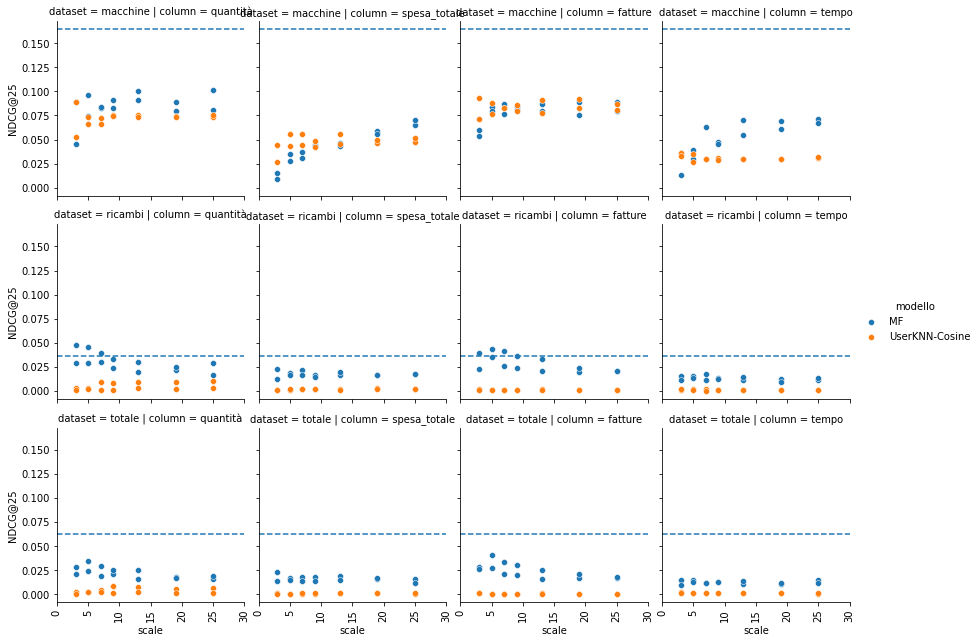
\includegraphics[width=16cm]{figures/risultati_ordered_globale.png}
    \captionof{figure}{Risultati ordered-based gruppo globale.}
    \label{tab:ordered_globale}
\end{center}

Abbiamo dei risultati positivi nelle matrici di tipo dataset ricambi e espressione d'interesse quantità e numero fatture.\\

\subsubsection{Tecnica ordered-based gruppo user-based}
Di seguito possiamo vedere i risultati relativi la tecnica ordered-based su gruppi di triplette appartenenti allo stesso user.
Il grafico composto \ref{tab:ordered_user_based} possiede la stessa struttura di quello (\ref{tab:ordered_globale}) del paragrafo precedente.
\begin{center}
    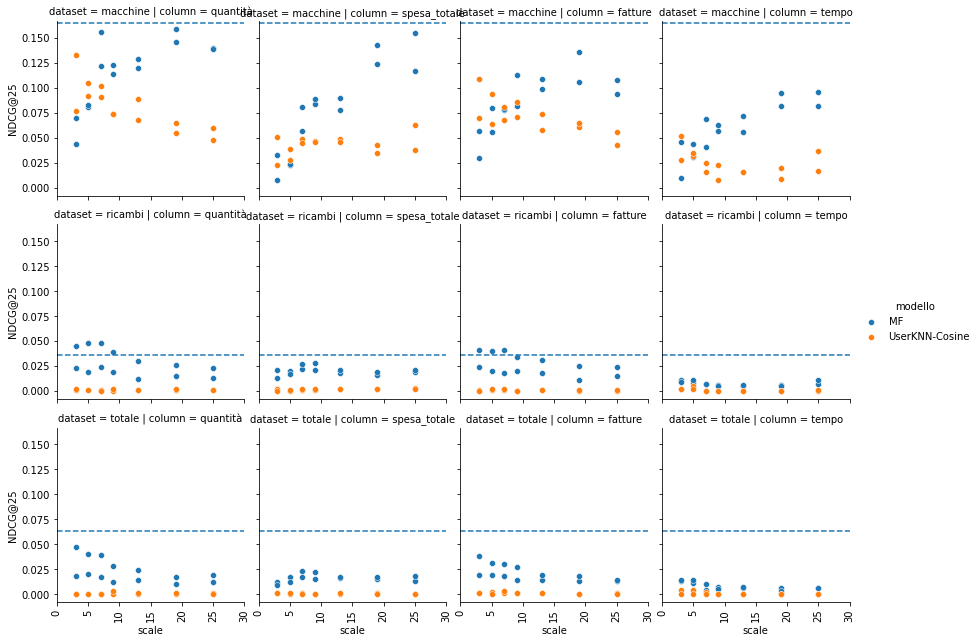
\includegraphics[width=16cm]{figures/risultati_ordered_singolo.png}
    \captionof{figure}{Risultati ordered-based gruppo user-based.}
    \label{tab:ordered_user_based}
\end{center}
Abbiamo qualche risultato positivo sempre per il tipo dataset ricambi con espressione d'interesse quantità e numero fatture, possiamo dire che siano leggermente peggiori dei precedenti.

\subsubsection{Tecnica ordered-based gruppo user-category-based}
Vediamo la tecnica di preprocessing ordered-based applicata al gruppo user-category-based, dove le triplette vengono divise per user e per categoria.
Le macchine hanno a disposizione solo la divisione in categorie secondo la gerarchia prodotto, mentre i ricambi possono essere divisi secondo le categorie di 2° e 3° livello della gerarchia prodotto e dal gruppo merceologico. Per il tipo dataset totale si proverà ad usare prima solo le categorie della gerarchia prodotto, poi le categorie della gerarchia prodotto solo per le macchine mentre per i ricambi le categorie del gruppo merceologico.

\paragraph{Macchine}\mbox{} \\
Come possiamo vedere dal grafico composto \ref{tab:ordered_macchine}, sulle righe abbiamo i livelli della gerarchia prodotto (1°, 2°, 3° livello), mentre sulle colonne abbiamo le espressioni d'interesse. 
Non sono presenti risultati che superino la soglia critica.
\begin{center}
    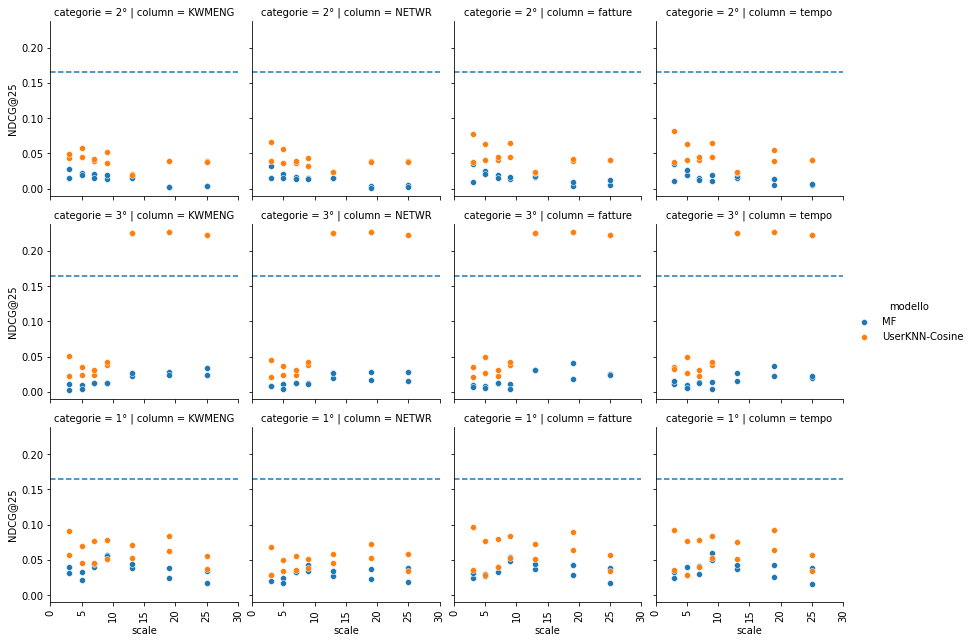
\includegraphics[width=16cm]{figures/risultati_ordered_categoria_macchine.png}
    \captionof{figure}{Risultati ordered-based gruppo user-category based dataset macchine.}
    \label{tab:ordered_macchine}
\end{center}

\paragraph{Ricambi}\mbox{} \\
Come possiamo vedere dal grafico composto \ref{tab:ordered_ricambi}, sulle righe abbiamo le categorie di 1° e 2° livello della gerarchia prodotto e la divisione del gruppo merceologico (\textit{MATKL}), mentre sulle colonne abbiamo le espressioni d'interesse. Abbiamo risultati che superano la soglia critica dividendo le triplette secondo le categorie di 2° e 3° livello con le espressioni quantità,numero fatture e recentezza.
\begin{center}
    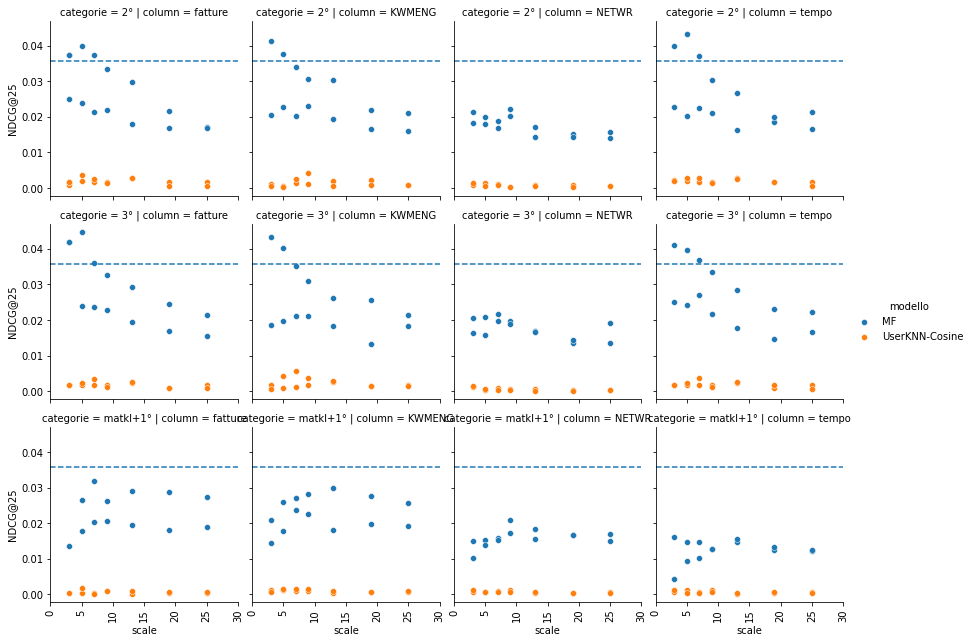
\includegraphics[width=16cm]{figures/risultati_ordered_categoria_ricambi.png}
    \captionof{figure}{Risultati ordered-based gruppo user-category based dataset ricambi.}
    \label{tab:ordered_ricambi}
\end{center}
\paragraph{Totale}\mbox{} \\
Come possiamo vedere dal grafico composto \ref{tab:ordered_totale}, sulle righe abbiamo il 1°, 2° e 3° livello della gerarchia prodotto e successivamente le precedenti categorie applicate solo alle macchine, mentre i ricambi si sono divisi secondo il gruppo merceologico. Sulle colonne abbiamo le espressioni d'interesse. Non abbiamo alcun risultato sopra la soglia.
\begin{center}
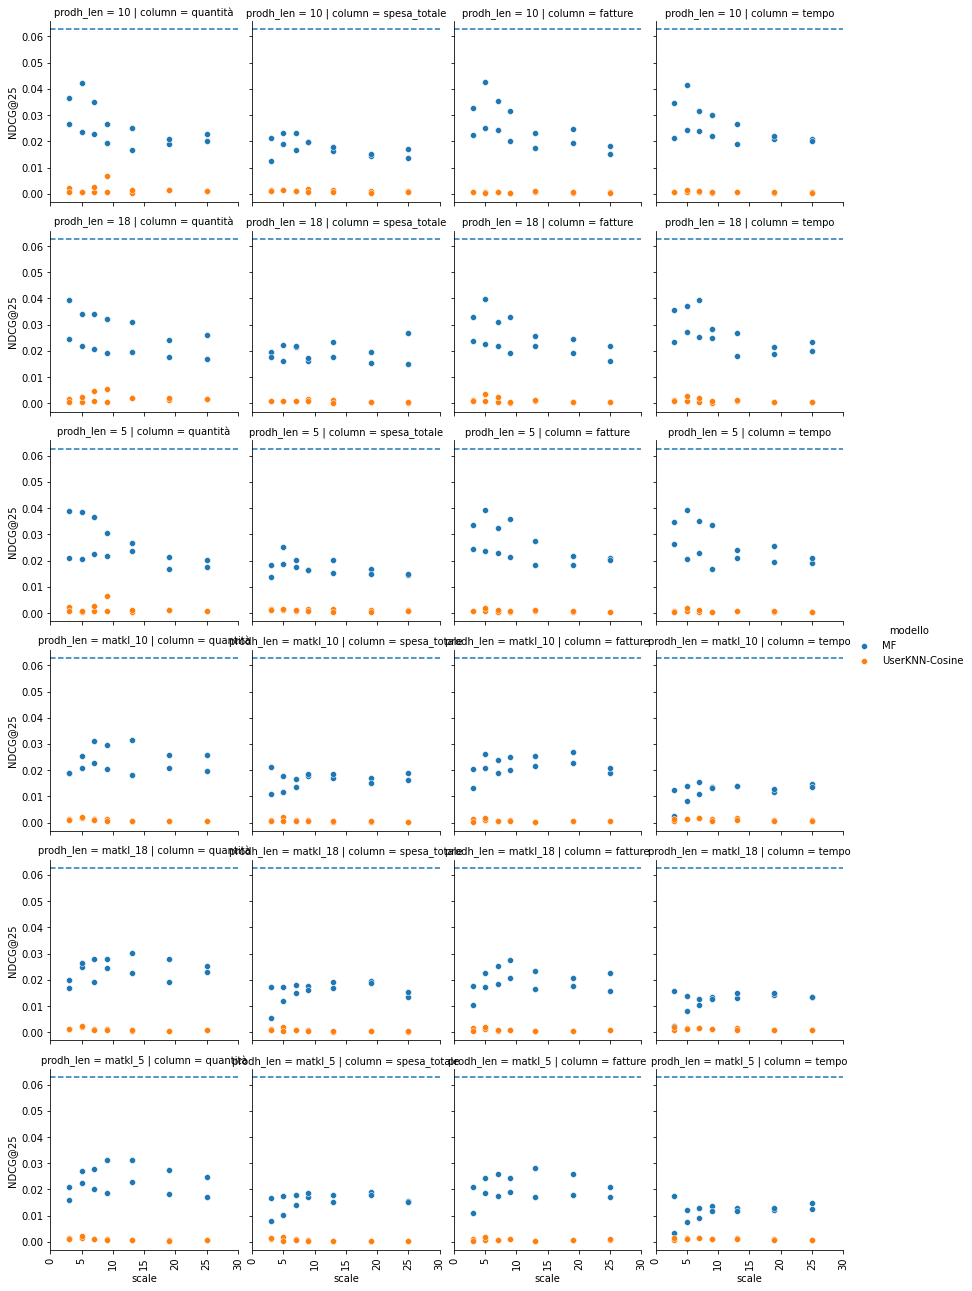
\includegraphics[width=14.5cm]{figures/risultati_ordered_categoria_totale.png}
\captionof{figure}{Risultati ordered-based gruppo user-category based dataset totale.}
\label{tab:ordered_totale}
\end{center}
%-------------------------------------------------------------------------------------------------------------------------------------------------------

\subsubsection{Tecnica product-based}
In questa sezione vedremo la tecnica di preprocessing product-based, dove si assegna ad ogni item lo stesso rating.
Nel grafico composto \ref{tab:product_based} possiamo vedere sulle righe i tipi di dataset (macchine, ricambi, totale), mentre sulle colonne le \textit{espressioni d'interesse}. Ciascun grafico poi mostra sulle ascisse la $scale$ della matrice dei rating e sulle ordinate il risultato ottenuto da tale matrice rispetto la metrica $NDCG@25$. 
La linea tratteggiata blu rappresenta il risultato del modello MostPop che viene usato come bound.
In questo grafico composto per ogni valore della scala vengono riportati quattro puntini, per questa tecnica ogni matrice dei rating è stata tenuta sia in versione continua che in versione intera. A queste due matrici vengono applicati i modelli MF e UserKnn, da cui otteniamo quattro risultati, quelli di colore blu sono i risultati forniti dal modello MF, mentre quelli arancioni quelli del modello UserKnn. Possiamo notare come questo approccio fornisca risultati positivi per ciascun tipo di dataset e per quasi tutte le espressioni d'interesse.
\begin{center}
    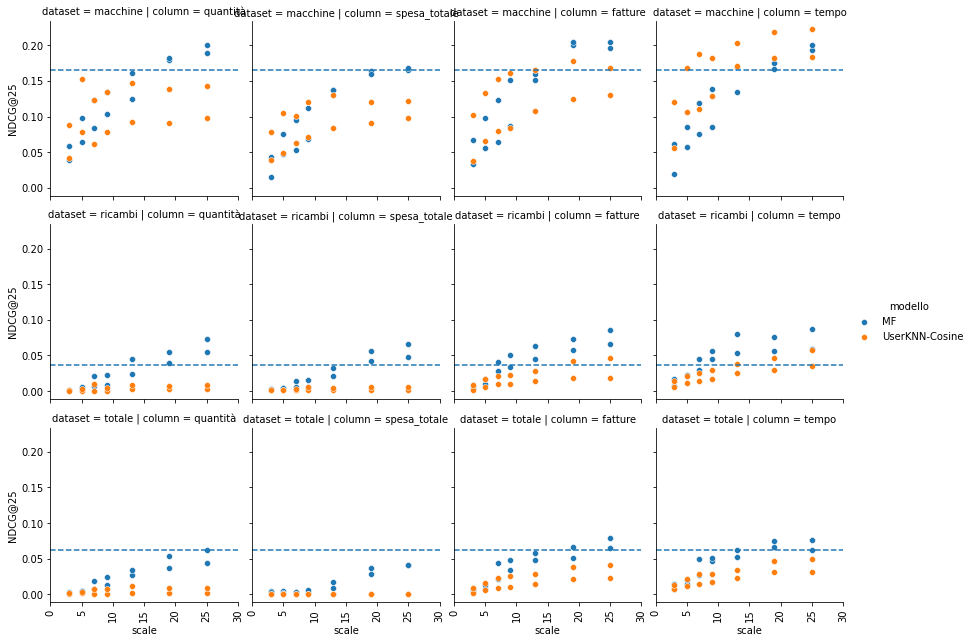
\includegraphics[width=15cm]{figures/prodotto.png}
    \captionof{figure}{Risultati tecnica product-based.}
    \label{tab:product_based}
\end{center}


\subsection{Fase test avanzata}
Per sintetizzare i risultati precedenti usiamo la tabella \ref{tab:fase_preliminare} dove sulle righe sono presenti i diversi metodi annessi ai gruppi e sulle colonne il tipo dataset, dov'è presente un 1 sappiamo che c'è stato almeno un risultato sopra la soglia.
\begin{center}
    \begin{tabular}{|l|ccc|}
        \toprule
        $tecniche$  & $macchine$ & $ricambi$ & $totale$   \\
        \midrule
        min-max globale             &   & 1 &   \\
        min-max user-based          &   & 1 &   \\
        min-max user-category-based &   & 1 &   \\
        \bottomrule
        ordered globale             &   & 1 &   \\
        ordered user-based          &   & 1 &   \\
        ordered user-category-based & 1 & 1 &   \\
        \bottomrule
        product-based               & 1 & 1 & 1  \\
        \bottomrule
    \end{tabular}
    \captionof{table}{Riassunto tecniche che hanno superato la fase preliminare per dataset.}
    \label{tab:fase_preliminare}
\end{center}
Se dovessimo stilare una classifica su questi risultati preliminari, potremmo affermare i seguenti punti:
\begin{itemize}
    \item la \textbf{tecnica product-based} funziona molto bene su tutti i dataset e finora ha restituito i risultati migliori;
    \item la \textbf{normalizzazione min-max} funziona solo sul tipo dataset ricambi, tra i tre gruppi quelli più efficaci sono quello user-based e user-category-based, sembra funzionare meglio su questo tipo di dataset rispetto la tecnica ordered-based;
    \item la \textbf{tecnica ordered-based} funziona sul tipo dataset macchine con il gruppo user-category-based ma risulta peggiore della tecnica product-based, mentre sul tipo dataset ricambi i gruppi che funzionano meglio sono quello globale e user-category-based.
\end{itemize}

Dopo aver visto i risultati delle tecniche nella fase preliminare, si passa alla fase avanzata selezionando tra tutte le matrici dei rating quelle che hanno ottenuto un valore della metrica superiore alla soglia critica data dal MostPop. \\
Per ciascuna combinazione di matrice dei rating e modello, che avesse restituito un risultato superiore a quello soglia, si è proceduto ad un tuning dei parametri. Una volta trovato quello migliore, in accordo al validation set, si è calcolato il risultato finale della metrica sul test set.
Nella fase avanzata il nuovo bound era quello del VAECF, vediamo ora i risultati del test set con relativa soglia.
\begin{center}
    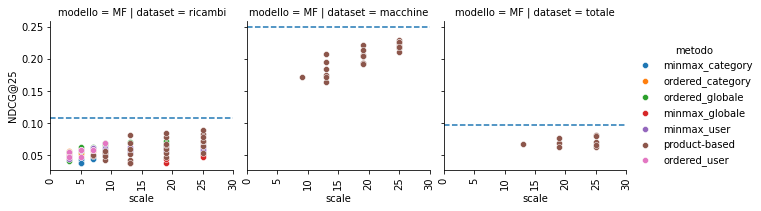
\includegraphics[width=16cm]{figures/validazione_mf.png}
    \captionof{figure}{Risultati MF ottimizzato su test set con matrici selezionate.}
    \label{tab:fase_avanzata_MF}
\end{center}
Nel grafico \ref{tab:fase_avanzata_MF} sono riportati i risultati ottenuti dai modelli MF ottimizzati sul test set. Nelle colonne troviamo rispettivamente il tipo dataset ricambi, macchine, totale con i loro relativi nuovi bound. Possiamo vedere in tutti e tre i grafici che i risultati non superano i valori soglia.
\begin{center}
    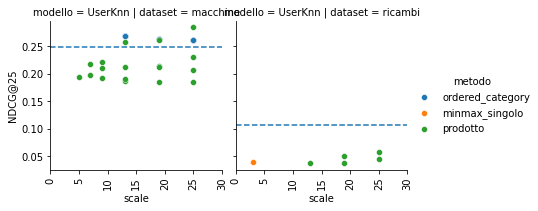
\includegraphics[width=16cm]{figures/validazione_userknn.png}
    \captionof{figure}{Risultati UserKnn ottimizzato su test set con matrici selezionate.}
    \label{tab:fase_avanzata_userknn}
\end{center}

Nel grafico \ref{tab:fase_avanzata_userknn} vengono mostrati i risultati ottenuti dai modelli UserKnn ottimizzati sul test set. Le colonne riportano rispettivamente il tipo dataset macchine e ricambi, possiamo vedere come il metodo product-based primeggi anche se ci sono due risultati della tecnica ordered-based, basata su categorie, oltre la soglia. Per il tipo dataset ricambi non c'è alcun risultato oltre la soglia.

Per quanto riguarda la distribuzione dei rating nelle matrici, quelle che hanno risultati superiori alla soglia hanno per circa il 66\% una distribuzione gaussian-like. Inoltre per quanto riguarda i valori della scala, i risultati migliori si sono ottenuti con il valore massimo di questa (25).\\
Vediamo ora i risultati finali sul test set per ogni tipo di dataset ndella tabella \ref{tab:risultati_finali}.
\begin{center}
    \begin{tabular}{|l|ccccc|}
        \toprule
        $dataset$  & $AUC$ & $NDCG@5$ & $NDCG@10$  & $NDCG@25$ & $NDCG@100$  \\
        \midrule
        macchine & 0.7288 & 0.1737 & 0.2223 & 0.2844 & 0.3203 \\
        ricambi  & 0.4930 &  0.0801 &    0.0919 &  0.1075 & 0.1401 \\
        totale  & 0.4343 &   0.0988  &  0.0874 &  0.0964 & 0.1398 \\
    \bottomrule
    \end{tabular}
    \captionof{figure}{Tabella risultati finali sul test set.}
    \label{tab:risultati_finali}
\end{center}
Riportiamo per ogni tipo di dataset tutte le informazioni relative alla matrice dei rating e alla tecnica con cui è stata generata, oltre che il modello utilizzato.\\
\begin{center}
    \begin{tabular}{|l|ccccc|}
        \toprule
        $dataset$  & $modello$ & tecnica &espressione interesse & scala & distribuzione  \\
        \midrule
        macchine & UserKnn& product-based &recentezza & 25 & gaussian-like   \\
        ricambi & VAECF& implicito &  & 1  &    \\
        totale & VAECF& implicito &  &  1 &     \\

    \bottomrule
    \end{tabular}
    \captionof{figure}{Informazioni sul modello e la tecnica dei risultati della tabella \ref{tab:risultati_finali}}
    \label{tab:info_finali}
\end{center}

\section{Risultati matrici grezze combinate}
Vediamo i risultati delle tecniche basate sulla combinazione delle matrici, si è utilizzato il validation set per il training e il test set per i risultati finali.
Entrambe le tecniche restituiscono risultati simili tra loro e di poco al di sotto di quelli ottenuti con le matrici singole. Nelle sezioni successive vedremo due grafici aventi sulle righe i tipi di dataset e sulle colonne le espressioni d'interesse. La linea tratteggiata è il bound dato dal VAECF sul test set.

\subsection{Combinazione liste \textit{TopN}}
Questa tecnica, nonostante nell'incrocio dataset macchine - tecnica product-based sembri funzionare, in realtà è stato fatto un test misurando il coefficiente di similarità delle liste $TopN$ prodotte da ciascun modello e si è visto che è quasi sempre molto alto. Quindi la combinazione delle liste non produce una lista così diversa da quelle di partenza. Vediamo i risultati nel grafico composto \ref{tab:risultati_finali_comb1}.
\begin{center}
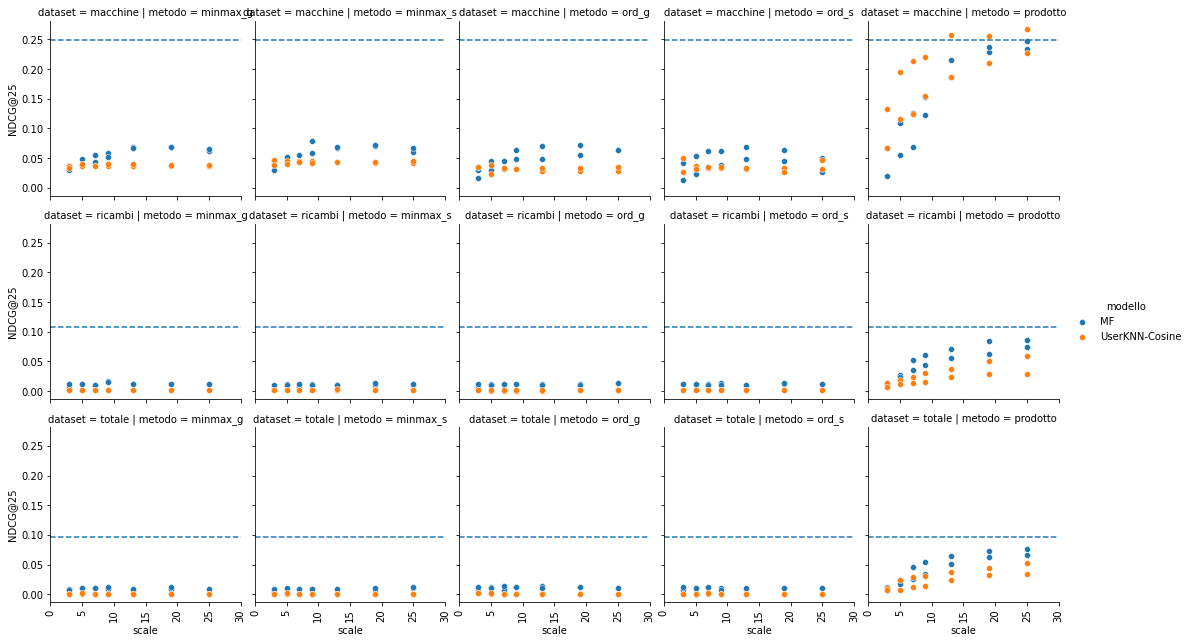
\includegraphics[width=16cm]{figures/comb_1.png}
\captionof{figure}{Grafico composto metodo basato su combinazione liste $TopN$.}
\label{tab:risultati_finali_comb1}
\end{center}
Nella tabella \ref{tab:risultati_finali_comb1_migliori} vediamo i risultati migliori per ciascun dataset sul test set, tutti forniti dalla tecnica product-based.
\begin{center}
    \begin{tabular}{|l|ccccc|}
        \toprule
        $dataset$ & $AUC$ & $NDCG@5$ & $NDCG@10$  & $NDCG@25$ & $NDCG@100$  \\
        \midrule
        macchine & 0.5658   &0.1516 & 0.2049 & 0.2683 & 0.3041 \\
        ricambi &  0.7873  &0.0756 & 0.0759 & 0.0865 & 0.1427 \\
        totale  & 0.7782   &0.0577 & 0.0648 & 0.0767 & 0.1273 \\
    \bottomrule
    \end{tabular}
\captionof{table}{Tabella risultati finali combinazione liste $TopN$.}
\label{tab:risultati_finali_comb1_migliori}
\end{center}

\subsection{Media matrici dei rating}
Il motivo per cui la versione basata sulle liste $TopN$ non funziona è che le liste di partenza non sono così diverse in quanto molte di esse si basano sull'ordinamento o su una normalizzazione su scala simile, la matrice media ottenuta sarà quindi molto simile a quelle di partenza.
\begin{center}
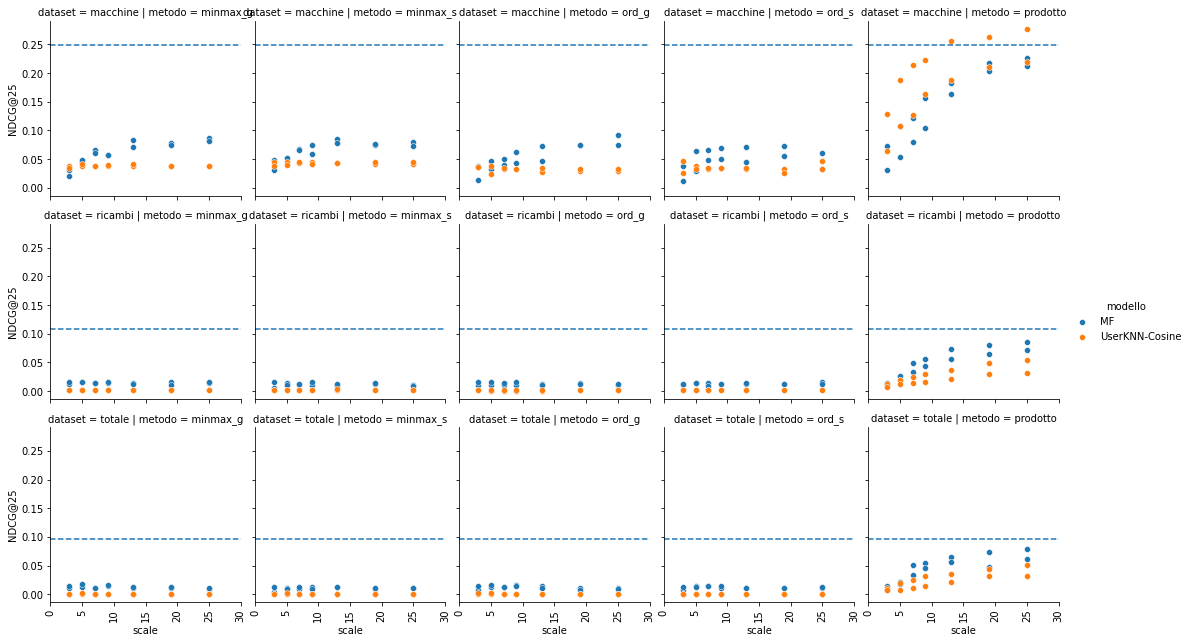
\includegraphics[width=16cm]{figures/comb_2.png}
\captionof{figure}{Grafico composto dei risultati metodo basato sula media matrici grezze.}
\label{tab:risultati_finali_comb2}
\end{center}
Nella tabella \ref{tab:risultati_finali_comb2_migliori} vediamo i risultati migliori per ciascun dataset sul test set.
\begin{center}
\begin{tabular}{|l|ccccc|}
    \toprule
    $dataset$  & $AUC$ & $NDCG@5$ & $NDCG@10$  & $NDCG@25$ & $NDCG@100$  \\
    \midrule
    macchine & 0.7288 & 0.1708 & 0.2149 & 0.2775 & 0.3133 \\
    ricambi & 0.8861  & 0.0757 & 0.0766 & 0.0860 & 0.1416 \\
    totale  & 0.8810  & 0.0605 & 0.0649 & 0.0792 & 0.1256 \\
\bottomrule
\end{tabular}
\captionof{table}{Tabella risultati finali del metodo basato su liste $TopN$ sul test set.}
\label{tab:risultati_finali_comb2_migliori}
\end{center}
\section{Risultati con approccio next-basket}
In questa sezione vedremo i risultati dell'approccio next-basket. Per prima cosa riportiamo quali sono stati i parametri selezionati con il tuning per ciascun dataset, riportati in tabella \ref{tab:next_basket_tuning}.\\

\begin{minipage}[H]{0.45\textwidth}
    \begin{center}

        \begin{tabular}{|l|ccc|}
            \toprule
            $dataset$ &    $\alpha$ &  $q$ & $r$ \\
            \midrule
            macchine & 0.5 & 100 & $\infty$ \\
            ricambi  &	0.75 & 50 & $\infty$ \\
            totale  & 0 & 100 & $\infty$ \\
        \bottomrule
        \end{tabular}
        \captionof{table}{Tabella paramentri selezionati.}
        \label{tab:next_basket_tuning}
    \end{center}
\end{minipage}
\begin{minipage}[H]{0.55\textwidth}
    Possiamo notare che alla fine il tuning ha portato ad avere una finestra di recentezza  $r = \infty$, quindi stiamo usando la popolarità \textit{popularity user-wise}. 
\end{minipage}\\

Possiamo inoltre vedere che la località $q$ è comunque alta mentre, per quanto riguarda $alpha$, osserviamo che nel dataset macchine si calcola la probabilità composta al 50\%. Nei ricambi si da più importanza a quella dello user in esame, ed infine nel totale si considera solo la probabilità composta dello user esterno.

Vediamo i risultati, in tabella \ref{tab:next_basket_val}, dei modelli ottimizzati sul validation set.
\begin{center}
    \begin{tabular}{|l|cccc|}
        \toprule
        $dataset$  &  $NDCG@5$ & $NDCG@10$  & $NDCG@25$ & $NDCG@100$  \\
        \midrule
        macchine & 0.5832 & 0.6278 & 0.6506 & 0.6627 \\
        ricambi & 0.1728 & 0.1892 & 0.2381 & 0.3317 \\
        totale  & 0.2196 & 0.2295 & 0.2834 & 0.3653 \\
    \bottomrule
    \end{tabular}
    \captionof{table}{Tabella risultati approccio next-based sul validation set.}
    \label{tab:next_basket_val}
\end{center}
E ora i corrispondenti risultati, in tabella \ref{tab:next_basket_test}, con il test set
\begin{center}
\begin{tabular}{|l|cccc|}
    \toprule
    $dataset$  &  $NDCG@5$ & $NDCG@10$  & $NDCG@25$ & $NDCG@100$  \\
    \midrule
    macchine & 0.6049 & 0.6476 & 0.6726 & 0.6741 \\
    ricambi & 0.2261 & 0.2403 & 0.2915 & 0.3811 \\
    totale  & 0.1955 & 0.2045 & 0.2595 & 0.3537 \\
\bottomrule
\end{tabular}
\captionof{table}{Tabella risultati approccio next-based sul test set.}
\label{tab:next_basket_test}
\end{center}
Ricordiamo che questi risultati non sono confrontabili con quelli delle sezioni precendenti, ma sono comunque molti interessanti.

\section{Confronto critico}
Il metodo di normalizzazione min-max non altera l'iniziale distribuzione dei valori, questi dopo essere stati scalati saranno per la maggior parte concentrati all'inizio dell'intervallo di rating. Questo fa sì che molti user abbiano solo item considerati pessimi, questo porta a similarità molto alta tra tutti gli user e non permette di distinguere gli item interessanti per esso. Il metodo in generale non funziona e non se ne raccomanda l'applicazione.\\
Il metodo ordered-based rispetto al precedente risolve molti problemi legati alla distribuzione dei rating, infatti ora la cardinalità di ciascun valore nella scala dei rating è circa uguale. La media dei rating degli user è collocala nella parte centrale della scala, mentre quella degli item copre tutta la scala, anche questo metodo non sembra funzionare proprio in virtù della variabilità dei rating per ogni item, anche se i risultati sono leggermente migliori dei precedenti.\\
Il metodo product-based assegnando ad un item lo stesso rating per tutti gli user ha fatto si che la media dei rating degli user non sia più centrata, in compenso però nella similarità è aiutata in quanto i rating di uno stesso item sono tutti uguali. Il suo funzionamento è molto legato alla popolarità rispetto le espressioni d'interesse e questo sembra aver dato risultati superiori rispetto ai precedenti, sicuramente la popolarità è uno degli ingredienti fondamentali per il raggiungimento degli obiettivi prefissati. In generale anche i risultati ottenuti con MostPop e VAECF sono bassi, possiamo quindi dire osservando i dati che il preprocessing sulle matrici grezze non funzioni e di riflesso neanche quello combinato che si basa su di esse. Lavorare sullo storico vendite con i precedenti metodi potrebbe non essere la strada giusta, con il metodo next-basket invece si sono ottenuti risultati promettenti anche se allenato su dataset più ristretti e per questo più incline ad ottenere risultati positivi. Il dataset tipo macchina è relativamete piccolo già di suo, quindi risulta ancora più facile ottenere buoni risultati, mentre quello totale funziona comunque peggio rispetto a quello di tipo ricambi, dall'unione di macchine e ricambi non sembra si possa ottenere quindi risultati positivi.
Ciò che si può concludere da questi test è che la popolarità giochi un ruolo importante nelle raccomandazioni e che l'approccio da seguire sia quello next-basket magari combinato con le espressioni d'interesse.